\begin{boxB}
    \lr{modAdd(a, b)}
    
    این تابع جمع ماژولار دو عدد 16 بیتی را محاسبه می کند.
    
    \lr{modMultiply(a, b)}
    
این تابع ضرب ماژولار دو عدد 16 بیتی را محاسبه می کند.

    \lr{plainSplit(x)}
    
این تابع یک عدد 64 بیتی را به چهار قسمت 16 بیتی تقسیم می کند و آنها را به عنوان خروجی برمی گرداند.


\lr{keyGeneration(k)}

این تابع یک کلید 128 بیتی را گرفته و با استفاده از توابع جانبی، 52 زیرکلید 16 بیتی را تولید می کند و آنها را در یک لیست برمی گرداند.

\lr{addInverse(k)}

این تابع معکوس جمع یک عدد 16 بیتی را محاسبه می کند.


\lr{multiplyInverse(a)}

این تابع معکوس ضرب یک عدد 16 بیتی را با استفاده از الگوریتم اقلیدس توانایی و قضایای نظریه اعداد، محاسبه می کند.

\lr{power(x, y, m)}

این تابع x به توان y را در حلقه ماژولار m با استفاده از الگوریتم توانایی سریع، محاسبه می کند.

\lr{gcd(a, b)}

این تابع بزرگترین مقسوم علیه مشترک دو عدد را با استفاده از الگوریتم اقلیدس، محاسبه می کند.

\lr{invKeyGeneration(k)}

این تابع لیست زیرکلید های k را گرفته و با استفاده از توابع جانبی، لیست زیرکلید های معکوس را برای فرآیند رمزگشایی، برمی گرداند.

\lr{round(p, k1, k2, k3, k4, k5, k6)}

این تابع یک دور از فرآیند رمزنگاری و رمزگشایی الگوریتم IDEA را پیاده سازی می کند. این تابع 6 زیرکلید و 64 بایت داده را در ورودی می گیرد و با استفاده از عمل های جمع، ضرب، XOR و جابجایی، خروجی 64 بایت داده را برمی گرداند.

\lr{finalRound(p, k1, k2, k3, k4)}

این تابع دور نهایی فرآیند رمزنگاری و رمزگشایی الگوریتم IDEA را پیدا سازید. این تابع 4 زیرکلید و 64 بایت داده را در ورودید میرید و با استفاده از عمل های جمع، ضرب و جابجایید خروجید 64 بایت داده را برمیریدانید.

\lr{encrypt(p, k)}

این تابع فرآیند کامل رمزنگارید الگوریتم IDEA را انجام میدهد. این تابع یک کلید 128 بیتی و 64 بایت داده را در ورودی می گیرد و با استفاده از توابع جانبی، خروجی 64 بایت داده رمزنگاری شده را برمی گرداند.

\lr{decrypt(c, k)}

این تابع فرآیند کامل رمزگشایی الگوریتم IDEA را انجام می دهد. این تابع یک کلید 128 بیتی و 64 بایت داده رمزنگاری شده را در ورودی می گیرد و با استفاده از توابع جانبی، خروجی 64 بایت داده رمزگشایی شده را برمی گرداند.


\end{boxB}

\begin{boxK}
    \lr{
        \lstinputlisting[language=Python]{Final/code/IDEA/encrypt.py}
    }
\end{boxK}

\begin{boxK}
    \lr{
        \lstinputlisting[language = Python]{Final/code/IDEA/decrypt.py}
    }
\end{boxK}

\begin{figure}[h]
    \centering
    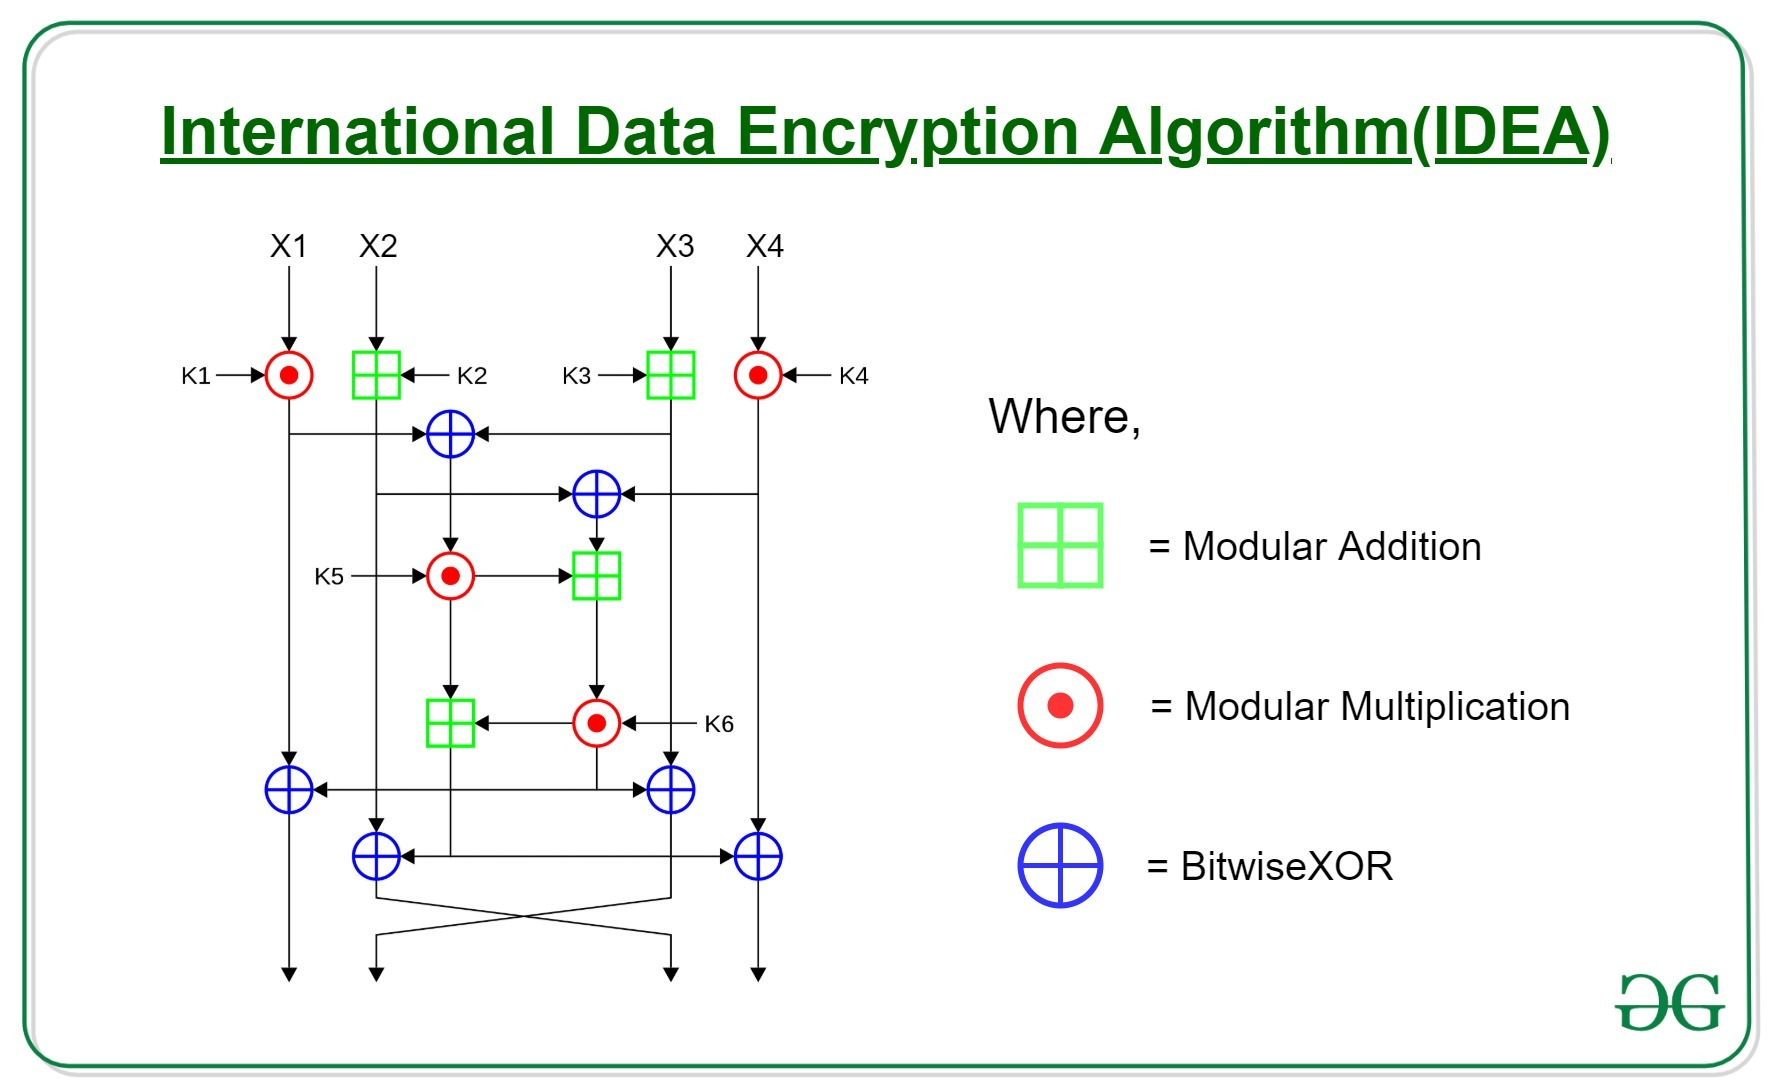
\includegraphics
    [width = 0.8\textwidth]
    {Final/images/IDEA.jpg}
    \caption{IDEA Algorithm}
    \label{fig:enter-label}
\end{figure}